%=================
\chapter{Sprint 2}
%=================


%------------------------
\section{Sprint Planning}
%------------------------
The first sprint resulted in a solid core for the utility. During the next sprint iteration, the core will be extended with more advanced functionality. After this sprint, the utility will have most of the functionalities it need to work in a real environment, and will probably be able to aid Thales in some of their operations.

Not yet understanding the complexity of all the requirements in the sprint backlog, the team ended in an uncertain person-hours estimate for some work objects. Time will show if we understood the complexity and assigned enough hours to implement it. The more complex, but not so critical functionalities will be part of sprint 3 and 4.   



\subsection{Duration}
%-----------------------
According to the work breakdown structure, \autoref{tab:wbs}, the planning meeting of the second sprint should have been conducted the 5th of October. After a request from the customer to see our planning for the second sprint at the weekly customer meeting, which was scheduled to be before our planning meeting the same day, we decided to advance the planning to the 4th of October. This is to maintain the good relationship to the customer and submit to their preference.

The sprint started with the planning meeting the 4th of October and our work started the following day. The sprint duration is 14 days, and will end the 18th of October with a review meeting.  

\subsection{Sprint Goal}
%-----------------------
The second sprint will build on the core created in the first sprint. During the sprint we will extend the functionality with more comprehensive and advanced features. Most of the requirements we intend to fulfill in this sprint had to be done subsequent to the first sprint, because the structure and design of the core had to be in place first. The requirements that are selected for this sprint is a natural advancement on the way to make the utility that the customer wants. 

One of the most crucial functions to work in a real environment, is the support for nested header-files. The handling of the \#include-statement gives the utility this feature. The goal of the sprint is to implement the \#include and mainly to have support for enums, bit streams, endianness and batch mode. 


\subsection{Back Log}
%-----------------------
The second sprint we will implement twelve requirements. Table
\ref{tab:sp2_req1b}-\ref{tab:sp2_req2d}  list each requirement with a time
estimate. \autoref{tab:sprint2req} is the sprint backlog for the first phase.
\autoref{tab:sprint2time} is the time table for the first phase.

\begin{table}[!ht] \small \center
\caption{Sprint 2 Requirement FR1-B\label{tab:sp2_req1b}}
\begin{tabular}{l l c}
	\toprule
	Requirement & Task & Hours \\
	\midrule
	\multirow{4}{5cm}{ Support members of type enum} & Design & 0 \\
	& Implementation & 3 \\
	& Testing & 3 \\
	& Documentation & 0 \\
	\bottomrule
\end{tabular}
\end{table}

\begin{table}[!ht] \small \center
\caption{Sprint 2 Requirement FR1-C\label{tab:sp2_req1c}}
\begin{tabular}{l l c}
	\toprule
	Requirement & Task & Hours \\
	\midrule
	\multirow{4}{5cm}{Support members of type struct} & Design & 0 \\
	& Implementation & 6 \\
	& Testing & 1 \\
	& Documentation & 0 \\
	\bottomrule
\end{tabular}
\end{table}

\begin{table}[!ht] \small \center
\caption{Sprint 2 Requirement FR1-F\label{tab:sp2_req1f}}
\begin{tabular}{l l c}
	\toprule
	Requirement & Task & Hours \\
	\midrule
	\multirow{4}{5cm}{Detect structs with same name} & Design & 0 \\
	& Implementation & 2 \\
	& Testing & 1 \\
	& Documentation & 0 \\
	\bottomrule
\end{tabular}
\end{table}

\begin{table}[!ht] \small \center
\caption{Sprint 2 Requirement FR2-B\label{tab:sp2_req2b}}
\begin{tabular}{l l c}
	\toprule
	Requirement & Task & Hours \\
	\midrule
	\multirow{4}{5cm}{Support display of structs within structs	} & Design & 0\\
	& Implementation & 5 \\
	& Testing & 6 \\
	& Documentation & 0 \\
	\bottomrule
\end{tabular}
\end{table}

\begin{table}[!ht] \small \center
\caption{Sprint 2 Requirement FR4-F\label{tab:sp2_req4f}}
\begin{tabular}{l l c}
	\toprule
	Requirement & Task & Hours \\
	\midrule
	\multirow{4}{5cm}{Support enumerated named values} & Design & 1 \\
	& Implementation & 1 \\
	& Testing & 2 \\
	& Documentation & 1 \\
	\bottomrule
\end{tabular}
\end{table}

\begin{table}[!ht] \small \center
\caption{Sprint 1 Requirement FR4-G\label{tab:sp2_req4g}}
\begin{tabular}{l l c}
	\toprule
	Requirement & Task & Hours \\
	\midrule
	\multirow{4}{5cm}{Support for bit strings} & Design & 2 \\
	& Implementation & 3 \\
	& Testing & 4 \\
	& Documentation & 1 \\
	\bottomrule
\end{tabular}
\end{table}

\begin{table}[!ht] \small \center
\caption{Sprint 2 Requirement FR1-E\label{tab:sp2_req1e}}
\begin{tabular}{l l c}
	\toprule
	Requirement & Task & Hours \\
	\midrule
	\multirow{4}{5cm}{Support members of type array} & Design & 0 \\
	& Implementation & 3 \\
	& Testing & 4 \\
	& Documentation & 0 \\
	\bottomrule
\end{tabular}
\end{table}

\begin{table}[!ht] \small \center
\caption{Sprint 2 Requirement FR4-E\label{tab:sp2_req4e}}
\begin{tabular}{l l c}
	\toprule
	Requirement & Task & Hours \\
	\midrule
	\multirow{4}{5cm}{Structs with various trailers} & Design & 3 \\
	& Implementation & 6 \\
	& Testing & 7 \\
	& Documentation & 2 \\
	\bottomrule
\end{tabular}
\end{table}

\begin{table}[!ht] \small \center
\caption{Sprint 2 Requirement FR4-B\label{tab:sp2_req4b}}
\begin{tabular}{l l c}
	\toprule
	Requirement & Task & Hours \\
	\midrule
	\multirow{4}{5cm}{Custom Lua configuration} & Design & 2 \\
	& Implementation & 5 \\
	& Testing & 9 \\
	& Documentation & 2 \\
	\bottomrule
\end{tabular}
\end{table}

\begin{table}[!ht] \small \center
\caption{Sprint 2 Requirement FR4-D\label{tab:sp2_req4d}}
\begin{tabular}{l l c}
	\toprule
	Requirement & Task & Hours \\
	\midrule
	\multirow{4}{5cm}{Dissector ID} & Design & 0 \\
	& Implementation & 1 \\
	& Testing & 1 \\
	& Documentation & 2 \\
	\bottomrule
\end{tabular}
\end{table}

\begin{table}[!ht] \small \center
\caption{Sprint 2 Requirement FR5-C\label{tab:sp2_req5c}}
\begin{tabular}{l l c}
	\toprule
	Requirement & Task & Hours \\
	\midrule
	\multirow{4}{5cm}{Endian handling} & Design & 0 \\
	& Implementation & 5 \\
	& Testing & 10 \\
	& Documentation & 0 \\
	\bottomrule
\end{tabular}
\end{table}

\begin{table}[!ht] \small \center
\caption{Sprint 2 Requirement FR6-C\label{tab:sp2_req6c}}
\begin{tabular}{l l c}
	\toprule
	Requirement & Task & Hours \\
	\midrule
	\multirow{4}{5cm}{Batch mode, folder support in the CLI} & Design & 0 \\
	& Implementation & 4 \\
	& Testing & 2 \\
	& Documentation & 1 \\
	\bottomrule
\end{tabular}
\end{table}


\begin{table}[!ht] \small \center
\caption{Sprint 2 Requirements\label{tab:sprint2req1}}
\begin{tabularx}{\textwidth}{l l X c c}
	\toprule
	& & & \multicolumn{2}{c}{Hours} \\
	\cmidrule(r){4-5}
	\# & Req. & Description & Est. & Act. \\
	\midrule
	1 & FR1-B & Support members of type enums & \underline{ 6 } & 5 \\
	   &  & Implementation			   	& 3 & 2\\
	   &  & Testing - unit				   	& 1 & 1\\
	   &  & Testing - end to end			& 2 & 2\\
	\addlinespace
	2 & FR1-C & Support members of type structs & \underline{ 7 } & 3.5  \\
	   &  & Implementation			   	& 6 & 3\\
	   &  & Testing - unit				   	& 1 & 0.5\\
	\addlinespace
	3 & FR1-F & Detect structs with same name & \underline{ 3 } &  3.5  \\
	   &  & Implementation			   	& 2 & 2.5\\
	   &  & Testing - unit				   	& 1 & 1\\
	\addlinespace
	4 & FR2-B & Support display of structs within structs & \underline{ 11 } &  -  \\
	   &  & Implementation			   	& 5 & 2\\
	   &  & Testing - unit				   	& 2 & 1\\
	   &  & Testing - end to end			& 4 & 2\\
	\addlinespace
	5 & FR4-F & Support enumerated named values  & \underline{ 5 } &  -  \\
	   &  & Design				   	& 1 & 0.5\\	   
	   &  & Implementation			   	& 1 & 0.5\\
	   &  & Testing - unit				   	& 1 & -\\
	   &  & Testing - end to end			& 1 & 1.5\\
	   &  & User documentation		   	& 1 & -\\
	\addlinespace
	6 & FR4-G & Support for bit strings & \underline{ 10 } & 11.5 \\
	   &  & Design				   	& 2 & 2\\	   
	   &  & Implementation			   	& 3 & 6\\
	   &  & Testing - unit				   	& 2 & 1\\
	   &  & Testing - end to end			& 2 & 1\\
	   &  & User documentation		   	& 1 & 1.5\\
	\bottomrule
\end{tabularx}
\end{table}

\begin{table}[!ht] \small \center
\caption{Sprint 2 Requirements continued\label{tab:sprint2req2}}
\begin{tabularx}{\textwidth}{l l X c c}
	\toprule
	& & & \multicolumn{2}{c}{Hours} \\
	\cmidrule(r){4-5}
	\# & Req. & Description & Est. & Act. \\
	\midrule
	7 & FR1-E & Support members of type array & \underline{ 7 } & 11 \\
	   &  & Implementation			   	& 3 & 6\\
	   &  & Testing - unit				   	& 1 & 1\\
	   &  & Testing - end to end			& 3 & 4\\
	\addlinespace
	8 & FR4-E & Structs with various trailers & \underline{ 18 } & - \\
	   &  & Design				   	& 3 & 2\\
	   &  & Implementation			   	& 6 & 4\\
	   &  & Testing - unit				   	& 2 & 1\\
	   &  & Testing - end to end			& 5 & -\\
	   &  & User documentation		   	& 2 & -\\
	\addlinespace
	9 & FR4-B & Support for custom Lua configuration & \underline{ 14 } & - \\
	   &  & Design				   	& 2 & -\\
	   &  & Implementation			   	& 5 & -\\
	   &  & Testing - unit				   	& 1 & -\\
	   &  & Testing - end to end			& 4 & -\\
	   &  & User documentation		   	& 2 & -\\
	\addlinespace
	10 & FR4-D & Dissector ID & \underline{ 4 } & - \\
	   &  & Implementation			   	& 1 & 1\\
	   &  & Testing - unit				   	& 1 & 1\\
	   &  & User documentation 			& 2 & -\\
	\addlinespace
	11 & FR5-C & Endian handeling & \underline{ 11 } & - \\
	   &  & Implementation			   	& 5 & -\\
	   &  & Testing - unit				   	& 2 & -\\
	   &  & Testing - end to end			& 6 & -\\
	\addlinespace
	12 & FR6-C & Batch mode; folder support in the CLI & \underline{ 7 } & - \\
	   &  & Implementation			   	& 4 & -\\
	   &  & Testing - unit				   	& 2 & -\\
	   &  & User documentation			& 1 & -\\
	\addlinespace
	13 & FR4-C & Support custom handeling of specific data types & \underline{ 5 } & - \\
	   &  & Implementation			   	& 2 & -\\
	   &  & Testing - unit				   	& 1 & -\\
	   &  & Testing - end to end			& 1 & -\\
	   &  & User documentation			& 1 & -\\
	\midrule
	& & Total: & 108  & - \\
	\bottomrule
\end{tabularx}
\end{table}



\begin{table}[!ht] \small \center
\caption{Sprint 2 Timetable\label{tab:sprint2time}}
\begin{tabularx}{\textwidth}{X c c}
	\toprule
	& \multicolumn{2}{c}{Hours} \\
	\cmidrule(r){2-3}
	Description & Est. & Act. \\
	\midrule
	Design & 30 & -\\
	\addlinespace
	Implementation & 44 & - \\
	\addlinespace
	Testing & 50 & -\\
	\addlinespace
	Documentation & 36 & -\\
	\midrule
	Total: &  & - \\
	\bottomrule
\end{tabularx}
\end{table}



%----------------------
\section{System Design}
%----------------------
For sprint 2 the team decided to refactor some of the code in order to make it easier to read and to split the functionalities of the utility in such a way that it reduces coupling within the system.Some new functionality was also added on the parser side in order to get the utility to recognize the datatypes mentioned in the sprint 2 backlog. Other than that, most of the design didn't change from sprint 1

\subsection{Utility}
%--------------------
\autoref{fig:sp2:class} shows the changes we made to the design for the utility for sprint 2. The main change was the creation of the wireshark module where the team gathered most of the functionality for creating dissector fields and looking up default C-types and their sizes. The developers also added new functionality to the config and dissector modules that handles the datatypes the utility was slated to support for sprint 2.
\begin{figure}[!htb]
	\center
	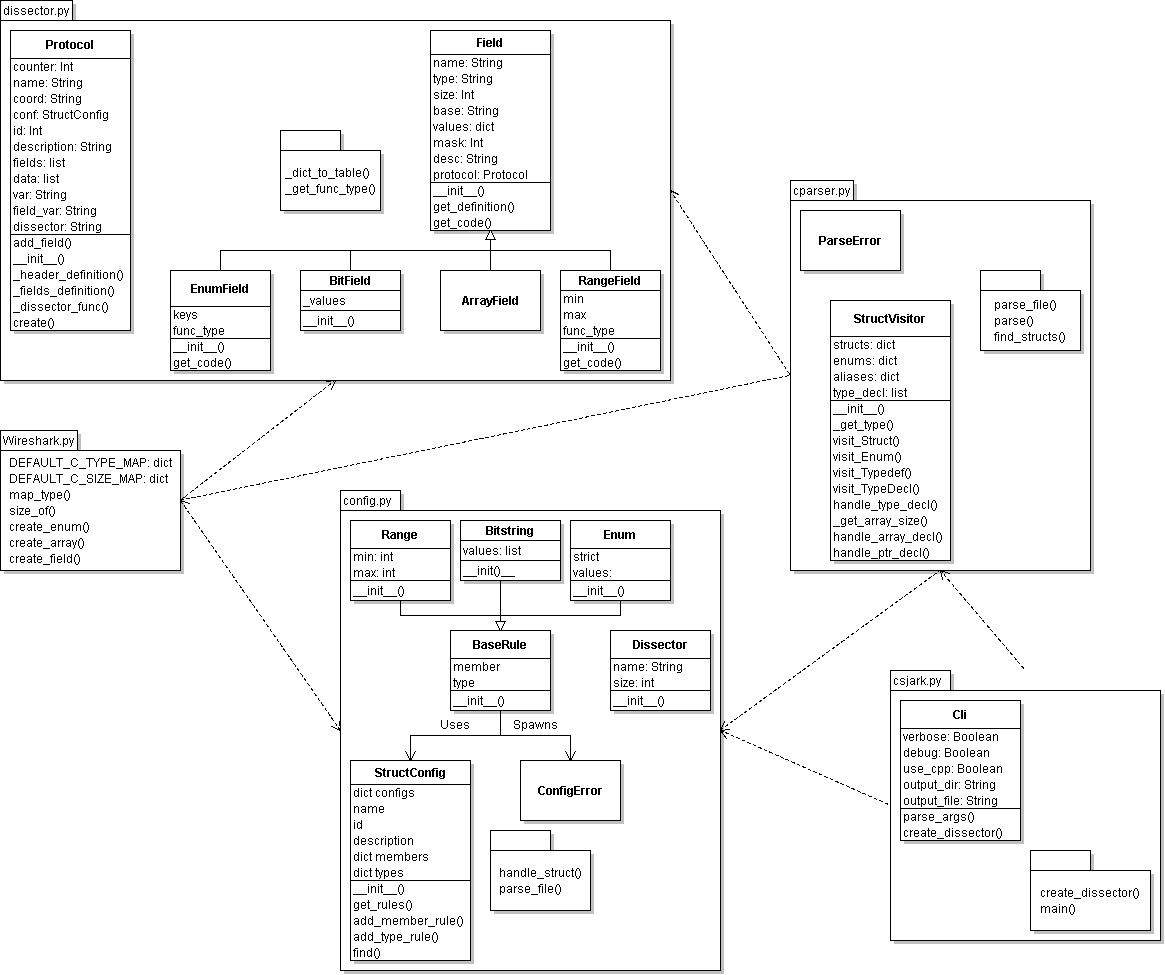
\includegraphics[width=\textwidth]{./sprints/img/class_diagram_s2}
	\caption{Class Diagram\label{fig:sp2:class}}
\end{figure}




%----------------------
\section{Implementation}
%----------------------

The previous sprint had a focus on creating a native implementation of the 
utility. In this sprint the focus has been on implementing data types for the 
C programming language and make it possible to configure more options on how 
the dissector will function. This section will cover the requirements 
implemented, how they are implemented and what the ''output'' look like.

\subsection{Support Members of Type enum}
%----------------------
\label{sec:support_enum}
Enum is a type declaration in C, which specifies enumeration constants.  Enum 
is supported because it is a basic datatype in the C language. 
\autoref{code:cenum} shows an example of an enum in a c-header file. The 
wireshark dissector will displayed the named value, because this will make it 
easier to read, an example is shown in \autoref{fig:wscenum}. The red 
rectangle show the enumerated named value.

\begin{figure}[ht]
	\center
	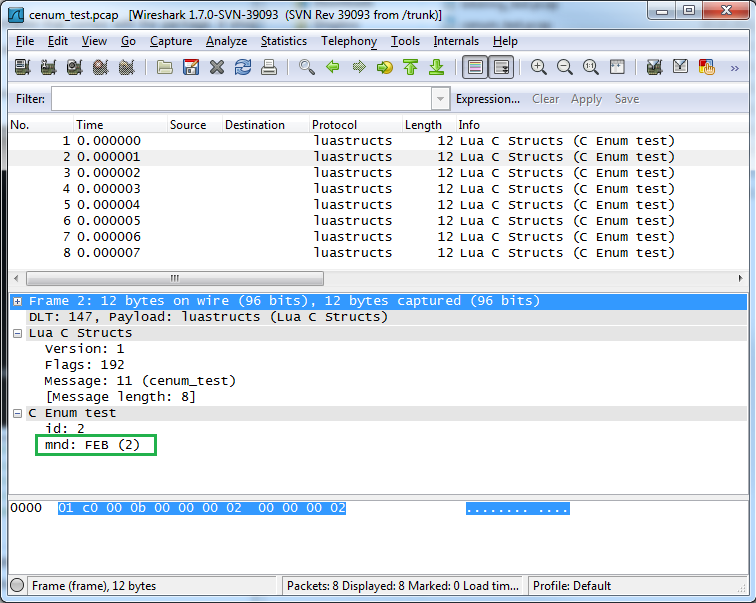
\includegraphics[width=\textwidth]{./sprints/img/wireshark_cenum}
	\caption{Class Diagram\label{fig:wscenum}}
\end{figure}

\lstset{language=C,caption={Enum support},label=code:cenum}
\lstinputlisting[language=C]{./sprints/code/cenum_test.h}

\subsection{Support Members of Type Struct}
%----------------------
Structs is an important part of the C language, a struct decalaration consists 
of a group of different fields, these fields can have any type, also struct. 
This was therfore a important requirement to implemented. An example is shown 
in \autoref{code:structmember}.

\lstset{language=C,caption={Struct support},label=code:structmember}
\lstinputlisting[language=C]{./sprints/code/struct_member.h}

\subsection{Detect Structs with Same Name}
%----------------------
It is possible that two structs can have the same name, therefore it is 
important to detect if there is more than one struct with the same name. If 
the parser finds two structs with the same name, an exception is 
raised, and the generation of the dissector is stopped.

\subsection{Support display of structs within structs}
%----------------------
TODO \autoref{fig:wsstructstruct}

\begin{figure}[ht]
	\center
	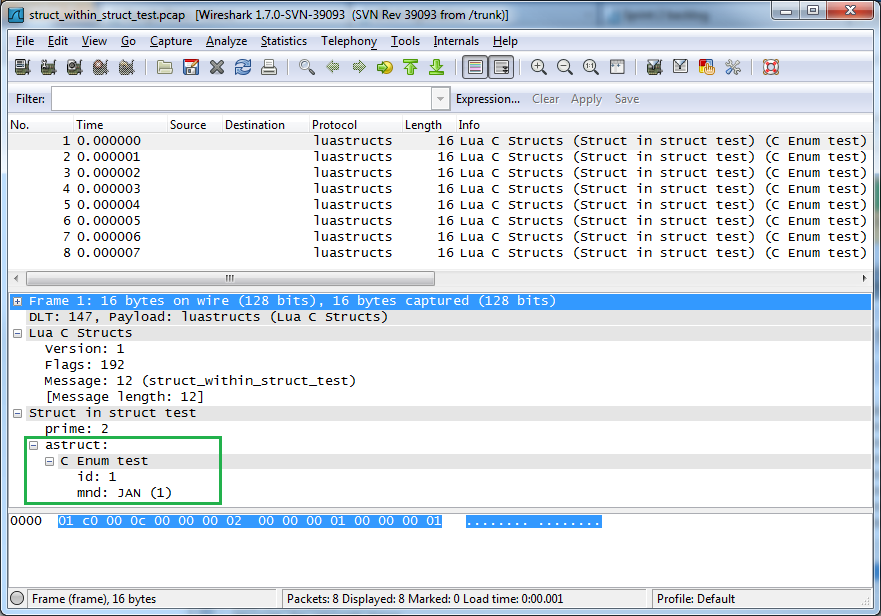
\includegraphics[width=\textwidth]{./sprints/img/wireshark_structwithstruct}
	\caption{Class Diagram\label{fig:wsstructstruct}}
\end{figure}

\subsection{Support Enumerated Named Values}
%----------------------
In C there is two ways to do enumerations, the first option was explained in 
\autoref{sec:support_enum}, the other way is to use \#define which is shown in 
\autoref{code:def_enum}. The advantage of using \#define is  that the values 
can be generated. Since this cannot be understand by the parser, it can be generated directly from the header file, so it have to 
be supported by configuration. \autoref{code:enum_conf}. The Lua-dissector 
will display the enum in the same way as in \autoref{sec:support_enum}.

\lstset{language=C,caption={Enumerated named values},label=code:def_enum}
\lstinputlisting[language=C]{./sprints/code/def_enum.h}

\lstset{language=C,caption={Enumerated named values config},label=code:enum_conf}
\lstinputlisting[language=C]{./sprints/code/def_enum.yml}

\subsection{Support for Bit Strings}
%----------------------
TODO

\subsection{Support Members of Type Array}
%----------------------
TODO

\subsection{Struct with Various Trailers}
%----------------------
TODO

\subsection{Custom Lua Configuration}
%----------------------
TODO

\subsection{Dissector ID}
%----------------------
TODO

\subsection{Endian Handling}
%----------------------
Endian handling is postponed to the next sprint, since it is a platform 
specified problem, and should be implemented togheter with platform support.

\subsection{Folder Support in the CLI}
%----------------------
TODO

\subsection{Support Custom Handling of Specified Data Types}
%----------------------
TODO

\subsection{Typedef Support}
%----------------------
TODO




%-----------------------
\section{Sprint Testing}
%-----------------------


%--------------------------
\section{Customer Feedback}
%--------------------------


%--------------------------
\section{Sprint Evaluation}
%--------------------------


